% 文档类(模板)
\documentclass[%
  type = bachelor,  % 本科论文(设计)
  % oneside,        % 单面模式
  twoside,          % 双面模式(openany)
]{nwafuthesis}
% 导言区

% 将需要载入的宏包统一在settings/package.tex中进行管理
% 请按自己的论文排版需求，加载需要的宏包

% TikZ绘图宏包
\usepackage{tikz}
% 卧图卧表宏包
\usepackage{lscape}
% 引号宏包
\usepackage{csquotes}
% 子图表宏包
\usepackage{subcaption}
% 双语标题宏包
\usepackage{bicaption}
% 合并表格行宏包
\usepackage{multirow}
% csv数据处理宏包
\usepackage{datatool}
% 单位符号宏包
\usepackage{siunitx}
% 跨页长表格宏包
\usepackage{longtable}
% 三线表宏包
\usepackage{booktabs}
% 新一代表格排版宏包
\usepackage{tabularray}
% 表格注释说明宏包
\usepackage{threeparttable}
% 带边框小页环境
\usepackage{boxedminipage2e}

\setCJKsansfont{SimHei}[AutoFakeBold=true] 
% 在导言区附近添加
\setCJKfamilyfont{kaitigb}{KaiTi_GB2312.ttf} % 定义楷体_GB2312字体族

%%% Local Variables:
%%% mode: latex
%%% TeX-master: "../main.tex"
%%% End:

% 将必要的设置统一在settings/format.tex中进行管理
\input{settings/format.tex}

% 编写测试文档用到的两个宏包，若不需要，可能删除
% 中文乱数假文宏包
\usepackage{zhlipsum}
% 最小工作示例(MWE)宏包，主要用于插图示例
\usepackage{mwe}

% 排版设置
\nwafuset{
% 论文格式
  style = {
    % font          = times*,           % 选择英文字体(需要安装有该字体，建议自动配置)
    % cjk-font      = adobe,            % 选择中文字体(需要安装有该字体，建议自动配置)
    hyperlink     = color,            % 超链接颜色
    % withchapter = false,            % 章标题是否为章模式(仅本科生需要)
    bib-resource  = {bib/sample.bib}, % 参考文献数据源文件名，注意需要完整路径及后缀名
    % anonymous = true,                 % 是否输出盲审格式论文
  },
% 信息录入
  info = {
    grade = {2022}, % 毕业年份(届)
    enroll = {2018}, % 入学年份(级)
    class-id = {1}, % 班级号
    btype = {paper}, % 本科类型(论文/设计)
    % btype = {design},
    title = { \nwafuthesis{}快速上手示例文档 }, % 中文题目
    title* = { \nwafuthesis{} Quick Start and Document Snippets }, % 英文题目
    department = { 信息工程学院 }, % 学院名称
    major = {计算机科学与技术}, % 专业
    author = { \TeX{}爱好者 }, % 作者中文名称
    supervisor = { 耿楠 }, % 指导教师
    cosupervisor = {Donald Knuth 大师}, % 协助指导教师
    date = {\datezh}, % 论文提交时间
    student-id = {202101000}, % 学号
    degree-title  = {工学学士},
  },
}
% 录入摘要
\nwafuset{
  abstract = {
    abstractfile  = { contents/chap00-abs-zh.tex }, % 中文摘要文件名称，注意需要有.tex后缀名
    abstractfile* = { contents/chap00-abs-en.tex }, % 英文摘要文件名称，注意需要有.tex后缀名
    keywords      = {学位论文, 模板, \nwafuthesis}, % 中文关键字列表，注意用英文逗号分隔。
    keywords*     = {NWAFU thesis, document class, space is accepted here}, % 英文关键字列表，注意用英文逗号分隔
  },
}

% ============================================================
% 封面第一页重定义（无学号，严格间距，黑体20号/二号/小三）
% ============================================================
\ExplSyntaxOn
\ctex_at_end_preamble:n
  {
    % 页面实例：无学号，增加英文标题，上方空 3 行
    \__nwafu_declare_page:nn { cover-i-default }
      {
        content     = { logo, type, title, en-title, simple-info },
        prefix      = cover / i /,
        top-skip    = 2\normalbaselineskip,
        bottom-skip = 0 pt plus 1 fill,
      }

    % logo 元素：下方空 1 行
    \__nwafu_declare_element:nn { cover / i / logo }
      {
        content     = \__nwafu_cover_logo:,
        bottom-skip = 1\normalbaselineskip,
        align       = center,
      }

    % type 元素：黑体 20pt，函数内部控制字体
    \__nwafu_declare_element:nn { cover / i / type }
      {
        content     = \__nwafu_cover_type:,
        % bottom-skip = 1\normalbaselineskip,
        align       = center,
      }

    % 中文标题：黑体二号加粗
    \__nwafu_declare_element:nn { cover / i / title }
      {
        content     = \l__nwafu_info_title_tl,
        format      = \sffamily \zihao{2} \bfseries,
        % bottom-skip = 1\normalbaselineskip,
        align       = center,
      }

    % 英文标题：Times New Roman 二号加粗，下方空 6 行
    \__nwafu_declare_element:nn { cover / i / en-title }
      {
        content     = \l__nwafu_info_title_en_tl,
        format      = \zihao{2} \bfseries,
        bottom-skip = 3\normalbaselineskip,
        align       = center,
      }

    % 作者+导师+日期：黑体小三，函数内部控制字体
    \__nwafu_declare_element:nn { cover / i / simple-info }
      {
        content     = \__nwafu_cover_simple_info:,
        bottom-skip = 0 pt,
        align       = center,
      }

    % ---------- 封面用到的内部函数 ----------

    % 届论文类型：黑体 20pt
    \cs_set_protected:Npn \__nwafu_cover_type:
      {
        \group_begin:
          \sffamily \fontsize{20pt}{28pt}\selectfont
          \l__nwafu_info_grade_tl 届
          \clist_item:Nn \c__nwafu_thesis_type_clist { \g__nwafu_thesis_type_int }
          \clist_item:Nn \c__nwafu_bachelor_type_clist { \l__nwafu_info_bachelor_type_int }
        \group_end:
      }

    % 作者、指导教师、日期：黑体小三，标签 8em 分散对齐，内容 10em 居中
    \cs_set_protected:Npn \__nwafu_cover_simple_info:
      {
        \group_begin:
          \centering
          \sffamily \zihao{-3}
          \makebox[6em][s]{作者} \c__nwafu_fwid_colon_tl \quad
          \makebox[6em][c]{
            \bool_if:NTF \l__nwafu_anonymous_bool
              { \c__nwafu_name_anonname_tl }
              { \l__nwafu_info_author_tl }
          }
          \par \vspace{1\normalbaselineskip}
          \makebox[6em][s]{指导教师} \c__nwafu_fwid_colon_tl \quad
          \makebox[6em][c]{
            \bool_if:NTF \l__nwafu_anonymous_bool
              { \c__nwafu_name_anonname_tl }
              { \l__nwafu_info_supervisor_tl }
          }
          \par \vspace{4\normalbaselineskip}
          \l__nwafu_info_date_tl
        \group_end:
      }
  }
\ExplSyntaxOff

% ============================================================
% 题名页详细信息系统重定义（黑体小三，1.5倍行距，日期上方3行）
% ============================================================
\ExplSyntaxOn
% 重新定义题名页页面实例，压缩间距
\ctex_at_end_preamble:n
  {
    \__nwafu_declare_page:nn { cover-ii-bachelor }
      {
        content     = { id, logo, type, title, en-title, detailed-info },
        prefix      = cover / ii /,
        top-skip    = 0pt,
        bottom-skip = 0pt,
      }
    % id 元素：无下划线
    \__nwafu_declare_element:nn { cover / ii / id }
      {
        content     =
          {
            \group_begin:
              \rmfamily\zihao{-4}
              \c__nwafu_name_student_id_tl \c__nwafu_fwid_colon_tl
              \bool_if:NTF \l__nwafu_anonymous_bool
                { \c__nwafu_name_anonid_tl }
                { \l__nwafu_info_student_id_tl }
            \group_end:
          },
        format      = ,
        bottom-skip = 1.5\normalbaselineskip,
        align       = right,
      }

    % logo 元素
    \__nwafu_declare_element:nn { cover / ii / logo }
      {
        content     = \__nwafu_cover_logo:,
        bottom-skip = 0.5\normalbaselineskip,
        align       = center,
      }
    % type 元素：黑体20号（与封面一致）
    \__nwafu_declare_element:nn { cover / ii / type }
      {
        content     = \__nwafu_cover_type:,
        format      = \sffamily \fontsize{20pt}{28pt}\selectfont,
        bottom-skip = 0.5\normalbaselineskip,
        align       = center,
      }
    % 中文标题：黑体二号加粗
    \__nwafu_declare_element:nn { cover / ii / title }
      {
        content     = \l__nwafu_info_title_tl,
        format      = \sffamily \zihao{2} \bfseries,
        bottom-skip = 0.5\normalbaselineskip,
        align       = center,
      }
    % 英文标题：二号加粗
    \__nwafu_declare_element:nn { cover / ii / en-title }
      {
        content     = \l__nwafu_info_title_en_tl,
        format      = \zihao{2} \bfseries,
        bottom-skip = 1.5\normalbaselineskip,
        align       = center,
      }
  }

% 信息函数（防止跨页，黑体小三）
\cs_set_protected:Npn \__nwafu_cover_detailed_info:
  {
    \group_begin:
      \centering
      \RenewDocumentCommand \small {} {}
      \sffamily \fontsize{15pt}{20pt}\selectfont
      \begin{tabular}{ @{} r @{\hspace{0.5em}} c @{\hspace{0.5em}} l @{} }
        \makebox[8em][s]{学生姓名} & ： &
        \makebox[12em][c]{
          \bool_if:NTF \l__nwafu_anonymous_bool
            { \c__nwafu_name_anonname_tl }
            { \l__nwafu_info_author_tl }
        } \\[0.6\normalbaselineskip]
        \makebox[8em][s]{指导教师} & ： &
        \makebox[12em][c]{
          \bool_if:NTF \l__nwafu_anonymous_bool
            { \c__nwafu_name_anonname_tl }
            { \l__nwafu_info_supervisor_tl }
        } \\[0.6\normalbaselineskip]
        \makebox[8em][s]{合作指导教师} & ： &
        \makebox[12em][c]{
          \bool_if:NTF \l__nwafu_anonymous_bool
            { \c__nwafu_name_anonname_tl }
            { \l__nwafu_info_cosupervisor_tl }
        } \\[0.6\normalbaselineskip]
        \makebox[8em][s]{申请学位类别} & ： &
        \makebox[12em][c]{\l__nwafu_info_degree_title_tl}
        \\[0.6\normalbaselineskip]
        \makebox[8em][s]{专业名称} & ： &
        \makebox[12em][c]{\l__nwafu_info_major_tl}
        \\[0.6\normalbaselineskip]
        \makebox[8em][s]{培养单位} & ： &
        \makebox[12em][c]{\l__nwafu_info_department_tl}
        \\[2\normalbaselineskip]      % 日期上方 2 行
        \multicolumn{3}{c}{\l__nwafu_info_date_tl}
      \end{tabular}
    \group_end:
  }
\ExplSyntaxOff

% 正文区(有且只能有一个)
\begin{document}
% 这个命令用来关闭版心底部强制对齐，
% 可以减少不必要的 underfull \vbox 提示，但会影响排版效果
% \raggedbottom

% 由于论文模板中已设计了自动排版封面、摘要、目录等功能，
% 因此，无需手动排版。

% 主体部分是论文的核心

\chapter{插图和附表清单}
\chapter{主要符号注释表}
\chapter{术语表}

\mainmatter

% 建议采用多文件编译的方式编写论文，
% 比较好的做法是把每一章放进一个单独的 tex 文件里，
% 并在这里用 \include 导入，如：
% 本文件是示例论文的一部分
% 论文的主文件是位于上级目录的 `main.tex`

\chapter{快速上手}

\section{欢迎}

欢迎使用\nwafuthesis{}，本文档将以简单示例的方式介绍如何利用\nwafuthesis{}
模板进行学位论文写作与排版。在此，本文假定学位论文作者已具备\LaTeX{}使用经
验，并具备使用搜索引擎解决常见问题的能力。

需要说明的是，本文档并非是一份\LaTeX{}零基础教程。如果是完完全全的新手，
建议先阅读相关入门文档，如大名鼎鼎的\enquote{lshort-zh-cn.pdf}
(\url{https://mirrors.tuna.tsinghua.edu.cn/CTAN/info/lshort/chinese/lshort-zh-cn.pdf})。
同时，对于中文文档的排版，必须熟读\CTeX{}宏集手册\enquote{ctex.pdf}
(\url{https://mirrors.tuna.tsinghua.edu.cn/CTAN/language/chinese/ctex/ctex.pdf})。
当然，网络上诸如耿楠录制的\LaTeX{}教学系列视频等入门教程多如牛毛，可以自行
选取学习。

\section{\LaTeX 环境准备}

由于\nwafuthesis{}基于\LaTeX3进行开发，用到了一些\LaTeX{}较新的特性和宏包，
该模板后期不支持2021以下\TeX{}发行版，请及时升级发行版并更新所有宏包。
例如，\TeX~Live2021或MiK~\TeX21.2之后的发行版。

该模板的测试主要是在\TeX~Live2021+Ubuntu 20.04平台完成，并且\TeX~Live的已
更新所有宏包。

关于\LaTeX{}发行版的安装，强烈建议仔细阅读大名鼎鼎的\enquote{install-latex-guide-zh-cn.pdf}
(\url{https://mirrors.tuna.tsinghua.edu.cn/CTAN/info/install-latex-guide-zh-cn/install-latex-guide-zh-cn.pdf.pdf})。

\section{模板使用}

\subsection{工作流}
使用{\nwafuthesis}模板排版学位论文的工作流如\ref{fig:workflow}所示。

\begin{figure}[!htb]
  \centering
  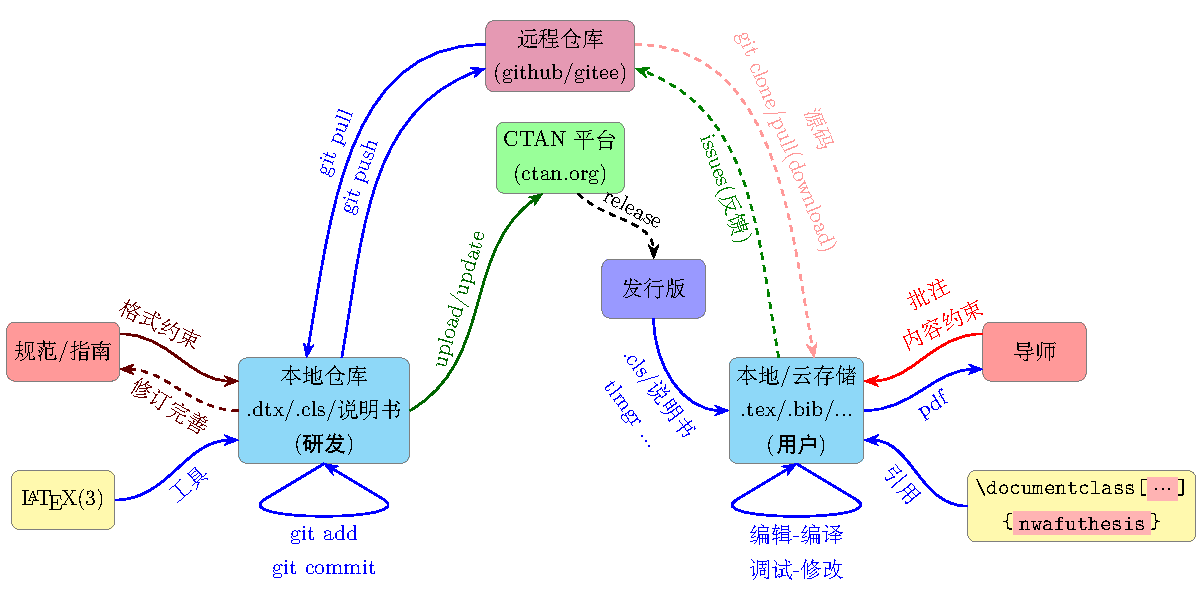
\includegraphics[width=0.85\textwidth]{figs/workflow}
  \caption{模板工作流}
  \label{fig:workflow}
\end{figure}

作为普通用户，仅需要通过{\LaTeX}发行版安装和更新模板，完成安装后，即可使用%
\verb|\documentclass{nwafuthesis}|载入该模板进行工作了。作为普通用户，
强烈建议只关心学位论文内容，通过与导师的反复沟通修改与完善论文内容即可。
关于学位论文排版格式问题应该交由开发者根据根据相关学校%
\emph{指南/规范}进行设计和调整。开发者完成模板开发及功能完善后，会上传到
CTAN(\url{www.ctan.org})，然后模板会被部署于{\LaTeX}发行版，此时普通
用户仅需要通过{\LaTeX}发行版的管理工具更新模板即可得到更新后的模板，
模板更新再次编译学位论文即可按最新的格式要求完成排版。

关于{\nwafuthesis}模板的使用的详细说明，一方面可以通过阅读其使用说明书和
写作样例进行学习，另一方面也可以参阅耿楠在B站发布的教学视频%
\url{https://www.bilibili.com/video/BV1tY4y1q7RT#reply107826496032}进行学习。

{\nwafuthesis}模板的源代码托管于\url{https://gitee.com/nwafu_nan/nwafuthesis-l3}，
如果有任何改进意见或者功能需求，欢迎前往 Gitee 仓库提交issue/PR，
以便进一步完善和美化我校学位论文\LaTeX{}模板。

\subsection{视觉识别系统图标}
论文写作时，请确认\textbf{论文的目录}(\verb|main.tex|所在的目录)下有
\enquote{logo/}文件夹，并内含以\enquote{nwafu-bar.pdf}和
\enquote{nwafu-circle.pdf}命名的最新版学校视觉识别系统矢量版图标文件。

如果论文目录下没有这些文件的话，请从本模板根目录复制一份。

\section{开始写作}

最方便的开始方法，莫过于修改现有的示例文稿，因此强烈推荐直接demo下的文
档实现学位论文撰写。

在撰写学位论文时，强烈建议按\ref{fig:dirforest}所示的目录结构组织和管理
写作过程中的各个文件：

\begin{figure}[!htb]
  \centering
  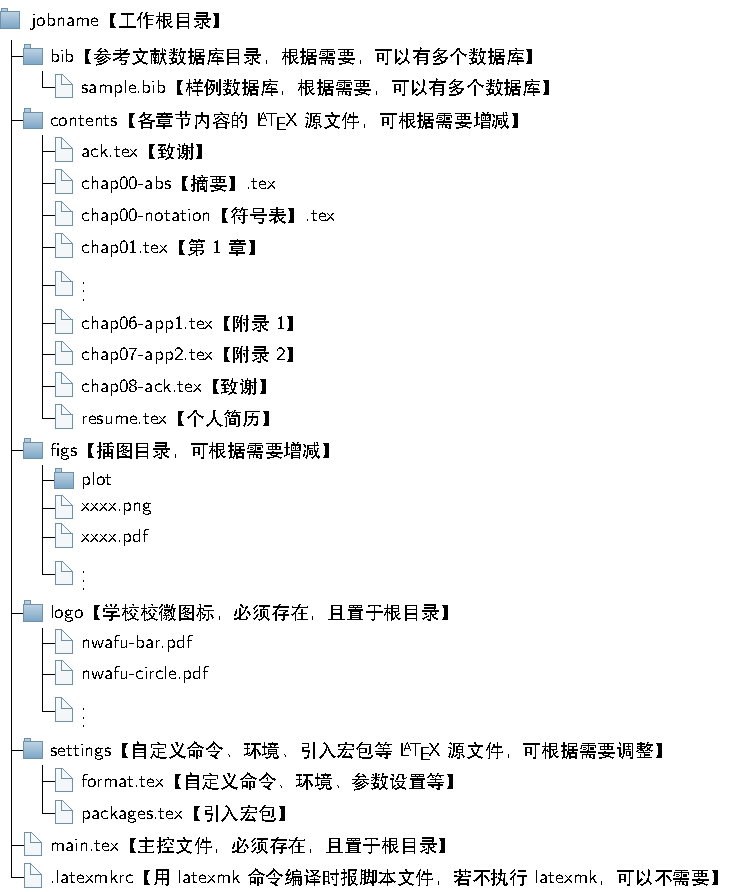
\includegraphics[width=0.60\textwidth]{figs/filestree}
  \caption{学位论文撰写目录结构}
  \label{fig:dirforest}
\end{figure}

完成部分或所有\verb|*.tex|撰写和修改后，可以在命令行使用 \verb|latexmk -xelatex main|
进行编译输出\verb|main.pdf|文件，可以根据需要对结果\texttt{pdf}文件进行改名。

也可以使用\texttt{TeXstudio}、\texttt{vscode}等GUI编辑器的进行编辑和编译输出。
关于这些编译器的配置和使用，请参阅相关说明资料。

\note{}由于\nwafuthesis{}需要处理图、表、公式及参考文献等交叉引用，因此，
往往需要多次编译才能得到正确的结果。为此，必须设置正确的编译方式和编译参数。
关于多次编译的问题，大家可以浏览耿楠在B站发布的视频
(\url{https://www.bilibili.com/video/BV1qa4y1v7my?spm_id_from=333.999.0.0})
进行学习。

\section{打印论文}

如果论文需要双面打印的话，请务必修改文档类选项，编译双面打印用的 PDF 文件。
具体地说，在主文件的头部，去除 \texttt{openany, oneside}，
改成 \texttt{twoside}。

同时，建议注释\cs{nwafuset}命令中的\enquote{style/hyperlink = color}，
以\emph{取消超链接颜色}。

%%% Local Variables:
%%% mode: latex
%%% TeX-master: "../main.tex"
%%% End:

% 本文件是示例论文的一部分
% 论文的主文件位于上级目录的 `main.tex`

\chapter{插图与表格}

在此，简单介绍一些学术论文中诸如插图、表格、数字与单位等排版元素的排版方法
及常用宏包的常用方法，希望能为读者写作时提供参考。

\section{插图}
\subsection{图片格式}
使用xelatex命令编译时，\LaTeX{}支持\verb|.pdf|和\verb|.eps|格式的矢量图，
也支持\verb|.jpg|、\verb|.png|或\verb|.bmp|格式的位图，当然也可以在\LaTeX{}
中直接绘图，关于插图图片推荐的方式有：

\begin{enumerate}
\item 使用其它绘图工具绘图生导出或打印成 \verb|pdf| 格式的\emph{矢量图}。
\item 使用\LaTeX{}的宏包来绘制插图，如 \pkg{Ti\textit{k}Z}，它兼容所有 \LaTeX{} 环境，
字体能与全文统一，质量最佳，但是需要的学习成本较大。
请务必先阅读 \pkg{Ti\textit{k}Z} 文档教程，
然后可以去 texample\footnote{\url{http://texample.net/tikz}} 等网站上找类似的例子，
\item 利用截图工具生成位图，不过\emph{质量堪忧}，小心遭批。
\item 对于现场照片等只能用相机等设备拍照成位图插入，小心遭批。
\item 最后，一般论文都是\emph{单色印刷}的，请确保插图在黑白打印情况下的清晰度。
\end{enumerate}

\begin{figure}[!htb]
  \centering
  \newcounter{density}
  \setcounter{density}{20}
  \input{figs/tikz_rot}
  \caption{在\LaTeX{}中直接用Ti\textit{k}Z绘制的矢量图}
  \label{fig:tikzrot}
\end{figure}

\begin{figure}[!htb]
  \centering
  
\includegraphics[width=4.1cm]{nwafu-circle}
  \caption{CorelDraw绘制导出的校徽PDF矢量图}
  \label{fig:logo}
\end{figure}

\subsection{插图浮动体}

由于学位论文中往往包含许多图片，为了保证较好的阅读体验，图片往往需要足够大，
而过大的图片有可能会带来分页困难，\LaTeX{}为此引入了\emph{浮动体}的机制，可
以令大块的内容脱离上下文，自动布置于合适的位置，从而避免在排版中产生留白
问题。对于插图，浮动体是通过\env{figure}环境实现的。同时，利用\env{figure}
环境还能够较好地实现插图编号及交叉引用的自动化，如\ref{fig:tikzrot}所示。关
于浮动体的细节，请参阅相关\LaTeX{}入门学习材料。

\subsection{子图排版}

如需要多个子图共用一个题注，需加载额外宏包，可以使用\pkg{subcaption}等宏包实现，
如\autoref{fig:sub2}所示。若需要更为复杂的子图控制，个人推荐使用\pkg{floatrow}
宏包实现更为复杂和灵活的子图排版中的细节控制。

\begin{figure}[!htb]
  \centering
  \subfloat[左边的大校徽\label{fig:sub1}]{
    
\includegraphics[width=2.8cm]{nwafu-circle}
  }\quad
  \subfloat[短标题：小校徽][小校徽，题注很长，不过请各位放心，它会自动换行\label{fig:sub2}]
  {
    
\includegraphics[width=4.6cm]{nwafu-bar}
  }
  \caption{用subcaption宏包排版子图}
  \label{fig:subfigs}
\end{figure}

强烈建议使用\emph{矢量图}图片，获得矢量图的一种方式是是直接使用
\LaTeX{}的绘制宏包\pkg{Ti\textit{k}Z}、\pkg{pgfplots}等宏包进行绘制，另一
种获取矢量图的方式是用Matplotlib、MatLab、Mathematica、Python等工具绘图后
导出pdf格式的矢量图。如\ref{fig:plots}所示。

\begin{figure}[htb]
  \centering
  \subfloat[二维图像\label{fig:func}]
    {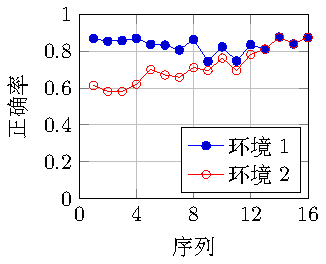
\includegraphics[scale=0.65]{figs/plot_2d}} \qquad
  \subfloat[三维图像\label{fig:sum}]
    {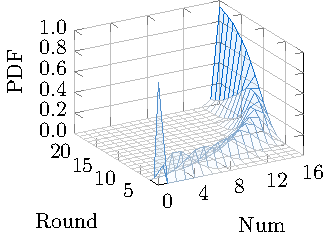
\includegraphics[scale=0.65]{figs/plot_3d}}
  \caption{利用 \pkg{pgfplot} 绘图}
  \label{fig:plots}
\end{figure}
%

\subsection{双语题注排版}

在研究生学位论文中，需使用双语题注(中文和英文)，为此，本模板选用
\pkg{bicaption}宏包实现双语题注，其效果可以参考\ref{fig:bicap}。当然，
也可以使用其它宏包实现双语题注排版，请大家根据情况自行处理。

\begin{figure}[!htb]
  \centering
  
\includegraphics[width=4.2cm]{nwafu-bar}
  \bicaption{双语题注}{bilingual caption}
  \label{fig:bicap}
\end{figure}

\subsection{超宽插图排版(卧图)}

如果需要插入图片超出了页面宽度，建议使用\emph{卧排}的方式实现排版，一种常
用的方式是使用 \pkg{lscape}宏包提供的 \env{landscape}环境进行排版。效果参
见\ref{fig:fullpage1}。

\setcounter{subfigure}{0}
\begin{landscape}
\vspace*{\fill} % 填充空白
\begin{figure}[!hb]
  \centering
  \subfloat[First caption\label{fig:fp1}]
    {
\includegraphics[width=.8\textheight]{nwafu-bar}} \\
  \subfloat[Second caption]
    {
\includegraphics[height=2cm]{nwafu-bar}}
  \caption{用\emph{卧排}实现超宽插图排版}
  \label{fig:fullpage1}
\end{figure}
\vspace*{\fill} % 填充空白
\end{landscape}

\section{表格}

\subsection{内置表格排版环境}

对于简单的表格，可以使用\LaTeX{}内置的 \env{tabular} 环境实现排版，
如\ref{tab:city}。

\begin{table}[htb]
  \centering
  \caption[城市人口]{城市人口数量排名 (source: Wikipedia)\label{tab:city}}
  \begin{tabular}{lr}
    \toprule
    \multicolumn{1}{c}{城市} & \multicolumn{1}{c}{人口} \\
    \midrule
    Mexico City              & 20,116,842               \\
    Shanghai                 & 19,210,000               \\
    Peking                   & 15,796,450               \\
    Istanbul                 & 14,160,467               \\
    \bottomrule
  \end{tabular}
\end{table}

\note{在学位论文中，表格要求采用三线表}，因此，需要使用\pkg{booktabs}宏包
提供的\cs{toprule}、\cs{midrule}和\cs{bottomrule}分别绘制表格的顶线、中线
和底线。

\subsection{表格浮动体}

由于学位论文中表格数量较多，且表格内容(长度)变化较大，当表格过长(一页内)时，
可能会带来分页困难，与插图类似，\LaTeX{}引入的\emph{浮动体}机制，可以使表格
脱离上下文，自动布置于合适的位置，从而避免在排版中产生留白问题。对于表格，
浮动体是通过\env{table}环境实现的。同时，利用\env{table}环境还能够较好地实
现插图编号及交叉引用的自动化。

\subsection{跨页长表格}

如果表格内容很多，导致无法放在一页内的话，则需要用 \env{longtable}宏包实现
表格的跨页排版，如\ref{tab:performance}所示(数据来自南京航空航天大学毕业论
文\LaTeX{}模板)。

% 定义表中用到的的宏，以简化表格代码并为后续修改提供统一接口
\def\tabcaption{实验数据}
\def\tabheadrow{
  \multirow{2}{*}{测试程序} & \multicolumn{1}{c}{正常运行} &
   \multicolumn{1}{c}{同步} & \multicolumn{1}{c}{检查点} &
   \multicolumn{1}{c}{卷回恢复} & \multicolumn{1}{c}{进程迁移} &
   \multicolumn{1}{c}{检查点} \\
   & \multicolumn{1}{c}{时间(s)} & \multicolumn{1}{c}{时间(s)} &
   \multicolumn{1}{c}{时间(s)} & \multicolumn{1}{c}{时间(s)} &
   \multicolumn{1}{c}{时间(s)} & \multicolumn{1}{c}{文件(KB)} \\
 }

% 定义跨页表续表表题
\def\ctntabcap{
   \caption* {表~\thetable\hskip1em 实验数据（续）}\\
   \addlinespace[-3.0ex]
 }
% 定义跨页表命令集合
\def\ctntabcmd{
   \ctntabcap\\
   \toprule
   \tabheadrow
   \midrule
   \endhead
   \midrule
   \multicolumn{7}{r}{\small 接下页}\\
   \endfoot
   \endlastfoot
 }

\begin{longtable}[c]{c*{6}{r}}
  \caption[实验数据]{\tabcaption}\label{tab:performance}\\
  \toprule
  \tabheadrow
  \midrule
  \endfirsthead
  \ctntabcmd
  CG.A.2 & 23.05 & 0.002 & 0.116 & 0.035 & 0.589 & 32491 \\
  CG.A.4 & 15.06 & 0.003 & 0.067 & 0.021 & 0.351 & 18211 \\
  CG.A.8 & 13.38 & 0.004 & 0.072 & 0.023 & 0.210 & 9890 \\
  CG.B.2 & 867.45 & 0.002 & 0.864 & 0.232 & 3.256 & 228562 \\
  CG.B.4 & 501.61 & 0.003 & 0.438 & 0.136 & 2.075 & 123862 \\
  CG.B.8 & 384.65 & 0.004 & 0.457 & 0.108 & 1.235 & 63777 \\
  MG.A.2 & 112.27 & 0.002 & 0.846 & 0.237 & 3.930 & 236473 \\
  MG.A.4 & 59.84 & 0.003 & 0.442 & 0.128 & 2.070 & 123875 \\
  MG.A.8 & 31.38 & 0.003 & 0.476 & 0.114 & 1.041 & 60627 \\
  MG.B.2 & 526.28 & 0.002 & 0.821 & 0.238 & 4.176 & 236635 \\
  MG.B.4 & 280.11 & 0.003 & 0.432 & 0.130 & 1.706 & 123793 \\
  MG.B.8 & 148.29 & 0.003 & 0.442 & 0.116 & 0.893 & 60600 \\
  LU.A.2 & 2116.54 & 0.002 & 0.110 & 0.030 & 0.532 & 28754 \\
  LU.A.4 & 1102.50 & 0.002 & 0.069 & 0.017 & 0.255 & 14915 \\
  LU.A.8 & 574.47 & 0.003 & 0.067 & 0.016 & 0.192 & 8655 \\
  LU.B.2 & 9712.87 & 0.002 & 0.357 & 0.104 & 1.734 & 101975 \\
  LU.B.4 & 4757.80 & 0.003 & 0.190 & 0.056 & 0.808 & 53522 \\
  CG.B.2 & 867.45 & 0.002 & 0.864 & 0.232 & 3.256 & 228562 \\
  CG.B.4 & 501.61 & 0.003 & 0.438 & 0.136 & 2.075 & 123862 \\
  CG.B.8 & 384.65 & 0.004 & 0.457 & 0.108 & 1.235 & 63777 \\
  MG.A.2 & 112.27 & 0.002 & 0.846 & 0.237 & 3.930 & 236473 \\
  MG.A.4 & 59.84 & 0.003 & 0.442 & 0.128 & 2.070 & 123875 \\
  MG.A.8 & 31.38 & 0.003 & 0.476 & 0.114 & 1.041 & 60627 \\
  MG.B.2 & 526.28 & 0.002 & 0.821 & 0.238 & 4.176 & 236635 \\
  MG.B.4 & 280.11 & 0.003 & 0.432 & 0.130 & 1.706 & 123793 \\
  LU.A.2 & 2116.54 & 0.002 & 0.110 & 0.030 & 0.532 & 28754 \\
  LU.A.8 & 574.47 & 0.003 & 0.067 & 0.016 & 0.192 & 8655 \\
  LU.B.2 & 9712.87 & 0.002 & 0.357 & 0.104 & 1.734 & 101975 \\
  LU.B.8 & 2444.05 & 0.004 & 0.222 & 0.057 & 0.548 & 30134 \\
  EP.A.2 & 123.81 & 0.002 & 0.010 & 0.003 & 0.074 & 1834 \\
  EP.A.8 & 31.06 & 0.004 & 0.017 & 0.005 & 0.073 & 1661 \\
  EP.B.2 & 495.49 & 0.001 & 0.009 & 0.003 & 0.196 & 2011 \\
  EP.B.8 & 126.74 & 0.003 & 0.017 & 0.005 & 0.083 & 1656 \\
  \bottomrule
\end{longtable}

\subsection{表格的双语题注}

在研究生学位论文中，需使用双语题注(中文和英文)，为此，本模板选用
\pkg{bicaption}宏包实现双语题注，其效果可以参考\ref{tab:bicap}。当然，
也可以使用其它宏包实现双语题注排版，请大家根据情况自行处理。

\begin{table}[htb]
  \centering
  \bicaption[城市人口]{城市人口数量排名 (source:
    Wikipedia)\label{tab:bicap}}{Urban population ranking}
  \begin{tabular}{lr}
    \toprule
    \multicolumn{1}{c}{城市} & \multicolumn{1}{c}{人口} \\
    \midrule
    Mexico City              & 20,116,842               \\
    Shanghai                 & 19,210,000               \\
    Peking                   & 15,796,450               \\
    Istanbul                 & 14,160,467               \\
    \bottomrule
  \end{tabular}
\end{table}

\subsection{超宽表格排版(卧表)}

如果需要插入超出页面宽度的表格，可以使用\pkg{lscape}宏包提供的 \env{landscape}
环境排版\emph{卧表}，效果参见\ref{tab:toowidetab}。

\begin{landscape}
\vspace*{\fill} % 填充空白
\begin{table}[!htb]
  \centering
  \caption{Laser specifications}
  \label{tab:toowidetab}
  \begin{tabular}{ccccccccc}
    \toprule
    Wavelength & Model & Package & Emmitter type & Manufacturer & Power (mW) & Iop (mA) & Ith (mA) & Vop (V)\\
    \midrule
    405 & DL-7386-101HG & TO-56 & single & sanyo & 50-70 & 70 & 35 & 4.8\\
    450 & PL 450 & TO-38 & single & osram & 50-90 & 120 & 30 & 5.5\\
    638 & ML520G54 & TO-56 & single & mitsubishi & 90-100 & 150 & 50 & 2.7\\
    655 &  DL-5147-242 & TO-56 & single & sanyo & 30-50 & 80 & 40 & 3.8\\
    \bottomrule
  \end{tabular}
\end{table}
\vspace*{\fill} % 填充空白
\end{landscape}

如果需要插入超宽超长表格，可以使用\pkg{lscape}宏包提供的 \env{landscape}
结合\env{longtable}环境排版\emph{跨页卧表}，效果参见\ref{tab:landscapeperformance}。

\begin{landscape} 
  \begin{longtable}[c]{c*{6}{r}}
    \caption[实验数据]{\tabcaption}\label{tab:landscapeperformance}\\
    \toprule
    \tabheadrow
    \midrule
    \endfirsthead
    \ctntabcmd
    CG.A.2 & 23.05 & 0.002 & 0.116 & 0.035 & 0.589 & 32491 \\
    CG.A.4 & 15.06 & 0.003 & 0.067 & 0.021 & 0.351 & 18211 \\
    CG.A.8 & 13.38 & 0.004 & 0.072 & 0.023 & 0.210 & 9890 \\
    CG.B.2 & 867.45 & 0.002 & 0.864 & 0.232 & 3.256 & 228562 \\
    CG.B.4 & 501.61 & 0.003 & 0.438 & 0.136 & 2.075 & 123862 \\
    CG.B.8 & 384.65 & 0.004 & 0.457 & 0.108 & 1.235 & 63777 \\
    MG.A.2 & 112.27 & 0.002 & 0.846 & 0.237 & 3.930 & 236473 \\
    MG.A.4 & 59.84 & 0.003 & 0.442 & 0.128 & 2.070 & 123875 \\
    MG.A.8 & 31.38 & 0.003 & 0.476 & 0.114 & 1.041 & 60627 \\
    MG.B.2 & 526.28 & 0.002 & 0.821 & 0.238 & 4.176 & 236635 \\
    MG.B.4 & 280.11 & 0.003 & 0.432 & 0.130 & 1.706 & 123793 \\
    MG.B.8 & 148.29 & 0.003 & 0.442 & 0.116 & 0.893 & 60600 \\
    LU.A.2 & 2116.54 & 0.002 & 0.110 & 0.030 & 0.532 & 28754 \\
    LU.A.4 & 1102.50 & 0.002 & 0.069 & 0.017 & 0.255 & 14915 \\
    LU.A.8 & 574.47 & 0.003 & 0.067 & 0.016 & 0.192 & 8655 \\
    LU.B.2 & 9712.87 & 0.002 & 0.357 & 0.104 & 1.734 & 101975 \\
    LU.B.4 & 4757.80 & 0.003 & 0.190 & 0.056 & 0.808 & 53522 \\
    LU.B.8 & 2444.05 & 0.004 & 0.222 & 0.057 & 0.548 & 30134 \\
    CG.B.2 & 867.45 & 0.002 & 0.864 & 0.232 & 3.256 & 228562 \\
    CG.B.4 & 501.61 & 0.003 & 0.438 & 0.136 & 2.075 & 123862 \\
    CG.B.8 & 384.65 & 0.004 & 0.457 & 0.108 & 1.235 & 63777 \\
    MG.A.2 & 112.27 & 0.002 & 0.846 & 0.237 & 3.930 & 236473 \\
    MG.A.4 & 59.84 & 0.003 & 0.442 & 0.128 & 2.070 & 123875 \\
    MG.A.8 & 31.38 & 0.003 & 0.476 & 0.114 & 1.041 & 60627 \\
    MG.B.2 & 526.28 & 0.002 & 0.821 & 0.238 & 4.176 & 236635 \\
    MG.B.4 & 280.11 & 0.003 & 0.432 & 0.130 & 1.706 & 123793 \\
    MG.B.8 & 148.29 & 0.003 & 0.442 & 0.116 & 0.893 & 60600 \\
    LU.A.2 & 2116.54 & 0.002 & 0.110 & 0.030 & 0.532 & 28754 \\
    LU.A.4 & 1102.50 & 0.002 & 0.069 & 0.017 & 0.255 & 14915 \\
    LU.A.8 & 574.47 & 0.003 & 0.067 & 0.016 & 0.192 & 8655 \\
    LU.B.2 & 9712.87 & 0.002 & 0.357 & 0.104 & 1.734 & 101975 \\
    LU.B.4 & 4757.80 & 0.003 & 0.190 & 0.056 & 0.808 & 53522 \\
    LU.B.8 & 2444.05 & 0.004 & 0.222 & 0.057 & 0.548 & 30134 \\
    EP.A.2 & 123.81 & 0.002 & 0.010 & 0.003 & 0.074 & 1834 \\
    EP.A.4 & 61.92 & 0.003 & 0.011 & 0.004 & 0.073 & 1743 \\
    EP.A.8 & 31.06 & 0.004 & 0.017 & 0.005 & 0.073 & 1661 \\
    EP.B.2 & 495.49 & 0.001 & 0.009 & 0.003 & 0.196 & 2011 \\
    EP.B.4 & 247.69 & 0.002 & 0.012 & 0.004 & 0.122 & 1663 \\
    EP.B.8 & 126.74 & 0.003 & 0.017 & 0.005 & 0.083 & 1656 \\
    \bottomrule
  \end{longtable}
\end{landscape}
\newpage

\subsection{表格自动生成}

也可以结合在\pkg{csvsimple}、\pkg{pgfplotstable}、\pkg{datatool}等宏包直接
使用逗号分隔的CSV文件中的数据生成\LaTeX{}表格。\ref{tab:datatooltab} 是将
\ref{tab:performance}中的数据存储在db.csv文件后，用\pkg{datatool}宏包实现
\LaTeX 表格排版的一个例子。

\DTLloaddb{ltab}{data/db.csv}% 可以在之前任何位置载入数据
\begin{longtable}[c]{c*{6}{r}}
  \caption[实验数据]{\tabcaption}\label{tab:datatooltab}\\
  \toprule
  \tabheadrow
  \midrule
  \endfirsthead
  \ctntabcmd
  \DTLforeach*{ltab}{\cola=cola, \colb=colb, \colc=colc, \cold=cold,
                     \cole=cole, \colf=colf, \colg=colg}%
        {\DTLiffirstrow{}{\tabularnewline}%
        \cola & \colb & \colc & \cold & \cole & \colf & \colg}\\ % 数据列位置可任意
  \bottomrule
\end{longtable}

在论文撰写中，应具备协作意识。排版是\LaTeX{}的事，而处理数据一定是
Excel等软件、R语言等开发语言的强项。这些数据处理的结果，
多数都可以非常方便的转存为逗号分隔的CSV数据文件。利用这个CSV数据实现表
格自动排版，让各类软件各负其责，通力合作才是高效工作之道。在一个软件里
干所有的事，不是好办法。

为减轻负担，在\nwafuthesis 模板并未直接引入这些CSV数据处理宏包，如果使用，
则需要手动载入需要的宏包，并通过查阅其使用说明学习宏包使用方法。
%
% \section{用\pkg{easyfloats}处理浮动体}
%
% 使用\LaTeX{}提供的\env{figure}和\env{table}浮动体环境，可以轻松实现浮动体排版。
% 但如果使用\pkg{easyfloats}宏包，则可以简化浮动体的语法，如所示。其使用细节可以
% 参考\url{https://latexstudio.net/index/details/index/mid/1181.html}中译说明。
%
% \emph{注意}：\pkg{easyfloats}宏包较新(2020.12.20)，需要注意更新宏包，
% 本示例文档中未给出示例代码。

\section{用tabularray宏包排版表格}

\pkg{tabularray} 是基于\LaTeX3设计的宏包，它不依赖其它宏包而实现排版，不仅
提供了基本表格排版功能，而且采用简便键值列表方式实现了表格的内容与格式分离。
该宏包被称为是新一代的表格排版，具体用法可见宏包的说明文档
(\url{https://mirrors.cqu.edu.cn/CTAN/macros/latex/contrib/tabularray/tabularray.pdf})。
耿楠完成了该说明文档的翻译
(\url{https://gitee.com/nwafu_nan/tabularray-doc-zh-cn/releases/2022A})。

\subsection{用\env{tblr}环境排版简单表格}

可以使用\pkg{tabularray}宏包提供的\env{tblr}环境排版简单表格，
如\ref{tab:tblr} 所示。

\begin{table}[htb]
  \caption{用tblr环境排版表格}
  \label{tab:tblr}
  \begin{tblr}{
    colspec = lcccc,
    cell{1}{1} = {r=2}{}, cell{1}{2,4} = {c=2}{},
    hline{1,Z} = {1pt, solid},
    hline{3} = {solid},
    hline{2} = {2-3}{},
    hline{2} = {4-5}{},
    cells = {font=\small},
  }
    Sample & I & & II & \\
    & A & B & C & D \\
    S1 & 5 & 6 & 7 & 8 \\
    S2 & 6 & 7 & 8 & 5 \\
    S3 & 7 & 8 & 5 & 6 \\
  \end{tblr}
\end{table}

\subsection{用\env{longtblr}环境排版跨页长表格}

可以使用\pkg{tabularray}宏包的\env{longtblr}环境实现长表格的跨页排版，但由
于本模板未对其格式进行详细设置，因此，需要使用其\cs{DefTblrTemplate}等命令
设置长表格的排版模式模板，建议将其置于导言区，以统一设置长表格排版格式，
然后再使用这些模板排版长表格。如\ref{tab:longtblr}所示。

\DefTblrTemplate{caption-tag}{default}{表\hspace{0.25em}\thetable}
\DefTblrTemplate{contfoot-text}{default}{接下页}
\DefTblrTemplate{caption-sep}{default}{\enskip}
\DefTblrTemplate{conthead-text}{default}{\!（续）}

\NewTblrTheme{fancy}{
  \SetTblrStyle{firsthead,mddlehead,lasthead}{font=\centering\small\sffamily}
  \SetTblrStyle{firstfoot}{font=\small}
  \SetTblrStyle{middlefoot}{font=\small}
  \SetTblrStyle{lastfoot}{font=\small}
}

\begin{longtblr}[
  theme = fancy,
  caption = {一个长长长长长长长长长的表格},
  entry = {短标题},
  label = {tab:longtblr},
  note{a} = {第一个表注。},
  note{$\dag$} = {第二个长长长长长长长的表注。},
  remark{注意} = {一些常规说明，一些常规说明，一些常规说明。},
  remark{来源} = {自力更生，自力更生，自力更生。},
]{
  colspec = {XXX}, width = 0.85\linewidth,
  rowhead = 1,
  hline{1,Z} = {1pt, solid},
  hline{2} = {solid},
  cells = {font=\small},
}
 Head    & Head  & Head    \\
 Alpha   & Beta  & Gamma   \\
 Epsilon & Zeta\TblrNote{a}       & Eta    \\
 Iota    & Kappa\TblrNote{$\dag$} & Lambda \\
 Nu      & Xi    & Omicron \\
 Rho     & Sigma & Tau     \\
 Phi     & Chi   & Psi     \\
 Alpha   & Beta  & Gamma   \\
 Epsilon & Zeta  & Eta     \\
 Iota    & Kappa & Lambda  \\
 Nu      & Xi    & Omicron \\
 Rho     & Sigma & Tau     \\
 Phi     & Chi   & Psi     \\
 Alpha   & Beta  & Gamma   \\
 Epsilon & Zeta  & Eta     \\
 Iota    & Kappa & Lambda  \\
 Nu      & Xi    & Omicron \\
 Rho     & Sigma & Tau     \\
 Phi     & Chi   & Psi     \\
 Alpha   & Beta  & Gamma   \\
 Epsilon & Zeta  & Eta     \\
 Iota    & Kappa & Lambda  \\
 Nu      & Xi    & Omicron \\
 Rho     & Sigma & Tau     \\
 Phi     & Chi   & Psi     \\
 Alpha   & Beta  & Gamma   \\
 Epsilon & Zeta  & Eta     \\
 Iota    & Kappa & Lambda  \\
 Nu      & Xi    & Omicron \\
 Rho     & Sigma & Tau     \\
 Phi     & Chi   & Psi     \\
\end{longtblr}


\subsection{用\env{booktabs}环境三线表}

如果在导言区使用\cs{UseTblrLibrary}命令引入\pkg{booktabs}，则该宏包可以通
过\env{booktabs}更为灵活的实现三线表的排版，如\ref{tab:booktabs}所示。

\begin{table}[htb]
  \caption{用tblr环境排版表格}
  \label{tab:booktabs}
  \begin{booktabs}{
    colspec = lcccc,
    cell{1}{1} = {r=2}{}, cell{1}{2,4} = {c=2}{},
    cells = {font=\small},
  }
    \toprule
    Sample & I & & II & \\
    \cmidrule[lr]{2-3} \cmidrule[lr]{4-5}
    & A & B & C & D \\
    \midrule
    S1 & 5 & 6 & 7 & 8 \\
    S2 & 6 & 7 & 8 & 5 \\
    S3 & 7 & 8 & 5 & 6 \\
    \bottomrule
  \end{booktabs}
\end{table}

\section{为表格添加数据来源说明}

对于学位论文，往往需要为表格添加数据来源说明及必要的其它注释说明。这可以
使用\pkg{tabularray}宏包的\env{longtblr}跨页长表格环境(\ref{tab:longtblr})
或\env{talltblr}浮动长表格环境实现，也可以通过\pkg{threeparttable}宏包实现。

\subsection{用tabularray宏包的talltblr环境添加数据来源说明}

\pkg{tabularray}宏包的\env{talltblr}环境可以实现可浮动长表格，并可以实现表
格题注和尾注排版，从而实现为表格添加数据来源说明，如\ref{tab:talltblr}

\begin{table}[htp]
  \begin{talltblr}[
    theme = fancy,
    caption = {用talltblr为表格添加脚注说明},
    entry = {短标题},
    label = {tab:talltblr},
    note{a} = {第一个表注。},
    note{$\dag$} = {第二个长长长长长长长的表注。},
    remark{注意} = {一些常规说明，一些常规说明，一些常规说明。},
    remark{来源} = {自力更生，自力更生，自力更生。},
  ]{
    colspec = {XXX}, width = 0.8\linewidth,
    hline{1,Z} = {1pt, solid},
    hline{2} = {solid},
    cells = {font=\small},
  }
    Alpha   & Beta  & Gamma                   \\
    Epsilon & Zeta  & Eta\TblrNote{a}         \\
    Iota    & Kappa & Lambda\TblrNote{$\dag$} \\
  \end{talltblr}
\end{table}

\subsection{用threeparttable宏包添加数据来源说明}
该宏包用于为表格添加脚注说明，如\ref{tab:threeparttable}。

\begin{table}[htp]
  \caption{用threeparttable为表格添加脚注说明}
  \label{tab:threeparttable}
  \begin{threeparttable}
    \begin{tabular}{c c c c}
      \toprule
      1st Column & 2nd Colimn & 
      3rd Colimn & 4th Colimn \\
      \midrule
      QWERTY\tnote{1} & test & test & test \\
      ASDFGH\tnote{2} & test & test & test \\
      \bottomrule
    \end{tabular}
    \begin{tablenotes}
      \item[1] 它来自太阳人;
      \item[2] 它来自月亮人
    \end{tablenotes}
  \end{threeparttable}
\end{table}

\section{图表浮动体}

浮动体是\LaTeX{}排版中的一个重要概念，在排版图表时，一定要使用插图和表格浮
动体实现排版，并用\cs{caption}命令添加题注以实现自动编号，\enquote{\emph{万万不可}}
强制进行手动编号，否则将会失去\enquote{自动化}功能，从而造成不必要的麻烦！

在\enquote{lshort-zh-cn.pdf}中有浮动体的详细说明，
在\url{https://www.latexstudio.net/archives/9786.html}
中也有浮动体使用技巧的说明，希望大家能够认真阅读并理解和掌握其使用方法和
技巧。

在撰写论文过程中，可以暂时不用考虑浮动体的浮动位置，等完全定稿后，现通过
调整图片大小、添加文字占空间、删减文字腾空间等方式细调图表等浮动体位置，
从而实现\emph{图表随文}的需求
(\url{https://ask.latexstudio.net/ask/article/79.html})。

\note{用浮动体、用浮动体、用浮动体}，重要的事要说三遍！一定要避免使用类似
\enquote{如下图}、\enquote{如右表}等这样的方式撰写学位论文。

另外，\env{longtable}和\env{longtblr}长表格环境不可用于浮动体环境。

\section{数字与国际单位}

本模板预加载 \pkg{siunitx} 来格式化文中的内联数字，该宏包有大量可定制的参数，
请务必阅读其文档，并在文档导言部分设置格式。

\begin{itemize}
  \item 旋转角度为 \ang{90}、\ang{270}
  \item 分辨率 \numproduct{1920 x 1080} 的像素数量约为 \num{2.07e6}
  \item 电脑显示器的像素间距为 \SI{1.8}{\nm}、\SI{180}{\um} 还是 \SI{18}{\mm}？
  \item 重力加速度 $g=\SI{9.8}{\kg\per\square\second}$、
  $g=\SI[inter-unit-product=\ensuremath{{}\cdot{}}]{9.8}{\kg\per\square\second}$，
  亦或 $g=\SI[per-mode=symbol]{9.8}{\kg\per\square\second}$
\end{itemize}

\section{中英文之间空格}

很遗憾，目前 \LaTeX{} 和 \CTeX{} 虽然能处理普通汉字与英文之间的间隔，
但是汉字与宏之间的空格仍然需要手工调整，请务必按以下的规则撰写原稿：
\begin{itemize}
  \item 如\ref{fig:sub2} 所示：\verb|如\ref{fig:sub2} 所示|，
      这个宏返回的是\enquote{图 x-xx}，所以前面两个汉字之间不能加空格，
      后面数字与汉字之间必须加空格；
  \item 距离为 1.7~个天文单位：\verb|距离为 1.7~个天文单位|，前面可以
      不加空格（\CTeX 会修正），后面必须加 \verb|~| 以防止在 \enquote{1.7}
      与\enquote{个}之间换行。此时更推荐写成 \SI{1.7}{au}：\verb|\SI{1.7}{au}|。
\end{itemize}

%%% Local Variables: 
%%% mode: latex
%%% TeX-master: "../main.tex"
%%% End:

% 本文件是示例论文的一部分
% 论文的主文件位于上级目录的 `main.tex`
\chapter{数学公式}

数学公式是\LaTeX{}排版中举世闻名的强项，关于数学公式的排版。在此，本文无意
展开讨论\LaTeX{}中的数学公式排版。只是重点说明一下由 \nwafuthesis{} 提供的
特有的宏。

\section{学习资源}

对于数学公式的排版在\enquote{lshort-zh-cn.pdf}的第四章给出了基本的使用方法，
请大家阅读学习。其内容对大多数人来说已经足够用了，但是如果不能解决问题的话
建议大家求助于搜索引擎或者有经验的人，这也不失为一个好办法。

常见的几个学习\LaTeX{}数学公式排版的资源链接如下：

\begin{itemize}
  \item 数学排版常见问题集:
        \url{https://www.latexstudio.net/index/details/index/mid/635}
  \item \pkg{amsmath}手册中译:
        \url{https://www.latexstudio.net/index/details/index/mid/706}
  \item \LaTeX{}公式备忘单:
        \url{https://www.latexstudio.net/index/details/index/mid/1052.html}
\end{itemize}

\section{公式排版与注解}

按我校学位论文排版要求，公式排版需要行间居中排版，公式编号按照一级标题(章)
连续编号(按章)并加小括号，不加导引线。类似这些细节\nwafuthesis{}模板都已进
行了设置。在撰写论文中只要将公式置于\env{equation}环境，并用\cs{label}命令
添加标签后用\cs{ref}或\cs{eqref}命令引用该公式即可。对于多行公式可以在
\env{equation}环境中使用\env{aligned}环境实现排版。

需要注意的是，公式解释下面的\enquote{式中}两字需要左起顶格编排，后接符号及
其解释；解释顺序为先左后右，先上后下；解释与解释之间用中文分号“；”分隔。
此时可以用\cs{noindent}命令临时取消首行缩进，在解释完公式符号后，再次正常
用空行进行分段便可自动恢复段落首行缩进。

例如：勾股定理可以表示为\ref{eq:gougu}

\begin{equation}
  a^2+b^2=c^2\label{eq:gougu}
\end{equation}

\noindent
式中，$a$是一条直角边边长；$b$是另一条直角边边长；$c$是斜边边长。

在公式解释结束后，段落缩进应复位至首行缩进2个汉字的模式。

\section{模板提供的数学环境}

\nwafuthesis{} 提供了一系列预定义的数学环境，详情见\nwafuthesis{}说明书的表6。
其使用样例有以下7种形式。

\subsection{axiom公理环境}

\begin{axiom}[欧几里得距离]
点$\mathbf{p}$与点$\mathbf{q}$的\textbf{欧几里德距离}，是连接两点的线段
($\overline{\mathbf{pq}}$)的长度。

在笛卡尔坐标系下，如果 $n$维欧几里得空间下的两个点 $\mathbf{p}=(p_1, p_2,
\dots, p_n)$ 与点$\mathbf{q} = (q_1, q_2, q_3, \dots, q_n)$，那么点$\mathbf{p}$
与点$\mathbf{q}$的距离，或者点$\mathbf{q}$与点$\mathbf{p}$的距离，由
\autoref{equ:1}定义：
\begin{align}
d(\mathbf{p},\mathbf{q}) = d(\mathbf{q},\mathbf{p}) & = \sqrt{(q_1-p_1)^2
                         + (q_2-p_2)^2 + \cdots + (q_n-p_n)^2} \notag \\
\label{equ:1}
& = \sqrt{\sum_{i=1}^n (q_i-p_i)^2}
\end{align}
\end{axiom}

\subsection{corollary推论环境}

\begin{corollary}[欧几里得距离]
点$\mathbf{p}$与点$\mathbf{q}$的\textbf{欧几里德距离}，是连接两点的线段
($\overline{\mathbf{pq}}$)的长度。

在笛卡尔坐标系下，如果 $n$维欧几里得空间下的两个点 $\mathbf{p}=(p_1, p_2,
\dots, p_n)$ 与点$\mathbf{q} = (q_1, q_2, q_3, \dots, q_n)$，那么点$\mathbf{p}$
与点$\mathbf{q}$的距离，或者点$\mathbf{q}$与点$\mathbf{p}$的距离，由
\autoref{equ:2}定义：
\begin{align}
d(\mathbf{p},\mathbf{q}) = d(\mathbf{q},\mathbf{p}) & = \sqrt{(q_1-p_1)^2
                         + (q_2-p_2)^2 + \cdots + (q_n-p_n)^2} \notag \\
\label{equ:2}
& = \sqrt{\sum_{i=1}^n (q_i-p_i)^2}
\end{align}
\end{corollary}

\subsection{definition定义环境}

\begin{definition}[欧几里得距离]
点$\mathbf{p}$与点$\mathbf{q}$的\textbf{欧几里德距离}，是连接两点的线段
($\overline{\mathbf{pq}}$)的长度。

在笛卡尔坐标系下，如果 $n$维欧几里得空间下的两个点 $\mathbf{p}=(p_1, p_2,
\dots, p_n)$ 与点$\mathbf{q} = (q_1, q_2, q_3, \dots, q_n)$，那么点$\mathbf{p}$
与点$\mathbf{q}$的距离，或者点$\mathbf{q}$与点$\mathbf{p}$的距离，由
\autoref{equ:3}定义：
\begin{align}
d(\mathbf{p},\mathbf{q}) = d(\mathbf{q},\mathbf{p}) & = \sqrt{(q_1-p_1)^2
                         + (q_2-p_2)^2 + \cdots + (q_n-p_n)^2} \notag \\
\label{equ:3}
& = \sqrt{\sum_{i=1}^n (q_i-p_i)^2}
\end{align}
\end{definition}

\subsection{example示例环境}

\begin{example}[欧几里得距离]
点$\mathbf{p}$与点$\mathbf{q}$的\textbf{欧几里德距离}，是连接两点的线段
($\overline{\mathbf{pq}}$)的长度。

在笛卡尔坐标系下，如果 $n$维欧几里得空间下的两个点 $\mathbf{p}=(p_1, p_2,
\dots, p_n)$ 与点$\mathbf{q} = (q_1, q_2, q_3, \dots, q_n)$，那么点$\mathbf{p}$
与点$\mathbf{q}$的距离，或者点$\mathbf{q}$与点$\mathbf{p}$的距离，由
\autoref{equ:4}定义：
\begin{align}
d(\mathbf{p},\mathbf{q}) = d(\mathbf{q},\mathbf{p}) & = \sqrt{(q_1-p_1)^2
                         + (q_2-p_2)^2 + \cdots + (q_n-p_n)^2} \notag \\
\label{equ:4}
& = \sqrt{\sum_{i=1}^n (q_i-p_i)^2}
\end{align}
\end{example}

\subsection{lemma引理环境}

\begin{lemma}[欧几里得距离]
点$\mathbf{p}$与点$\mathbf{q}$的\textbf{欧几里德距离}，是连接两点的线段
($\overline{\mathbf{pq}}$)的长度。

在笛卡尔坐标系下，如果 $n$维欧几里得空间下的两个点 $\mathbf{p}=(p_1, p_2,
\dots, p_n)$ 与点$\mathbf{q} = (q_1, q_2, q_3, \dots, q_n)$，那么点$\mathbf{p}$
与点$\mathbf{q}$的距离，或者点$\mathbf{q}$与点$\mathbf{p}$的距离，由
\autoref{equ:5}定义：
\begin{align}
d(\mathbf{p},\mathbf{q}) = d(\mathbf{q},\mathbf{p}) & = \sqrt{(q_1-p_1)^2
                         + (q_2-p_2)^2 + \cdots + (q_n-p_n)^2} \notag \\
\label{equ:5}
& = \sqrt{\sum_{i=1}^n (q_i-p_i)^2}
\end{align}
\end{lemma}

\subsection{proof证明环境}

\begin{proof}[欧几里得距离]
点$\mathbf{p}$与点$\mathbf{q}$的\textbf{欧几里德距离}，是连接两点的线段
($\overline{\mathbf{pq}}$)的长度。

在笛卡尔坐标系下，如果 $n$维欧几里得空间下的两个点 $\mathbf{p}=(p_1, p_2,
\dots, p_n)$ 与点$\mathbf{q} = (q_1, q_2, q_3, \dots, q_n)$，那么点$\mathbf{p}$
与点$\mathbf{q}$的距离，或者点$\mathbf{q}$与点$\mathbf{p}$的距离，由
\autoref{equ:6}定义：
\begin{align}
d(\mathbf{p},\mathbf{q}) = d(\mathbf{q},\mathbf{p}) & = \sqrt{(q_1-p_1)^2
                         + (q_2-p_2)^2 + \cdots + (q_n-p_n)^2} \notag \\
\label{equ:6}
& = \sqrt{\sum_{i=1}^n (q_i-p_i)^2}
\end{align}
\end{proof}

证明与其他定理环境稍有不同， 末尾会有一个 QED 符号。

\subsection{theorem定理环境}

\begin{theorem}[欧几里得距离]
点$\mathbf{p}$与点$\mathbf{q}$的\textbf{欧几里德距离}，是连接两点的线段
($\overline{\mathbf{pq}}$)的长度。

在笛卡尔坐标系下，如果 $n$维欧几里得空间下的两个点 $\mathbf{p}=(p_1, p_2,
\dots, p_n)$ 与点$\mathbf{q} = (q_1, q_2, q_3, \dots, q_n)$，那么点$\mathbf{p}$
与点$\mathbf{q}$的距离，或者点$\mathbf{q}$与点$\mathbf{p}$的距离，由
\autoref{equ:7}定义：
\begin{align}
d(\mathbf{p},\mathbf{q}) = d(\mathbf{q},\mathbf{p}) & = \sqrt{(q_1-p_1)^2
                         + (q_2-p_2)^2 + \cdots + (q_n-p_n)^2} \notag \\
\label{equ:7}
& = \sqrt{\sum_{i=1}^n (q_i-p_i)^2}
\end{align}
\end{theorem}


\section{交叉引用}

与图表一样，公式、定理等也需要采用专用的命令或环境进行排版以实现
编号、交叉引用等\emph{自动化}处理，\emph{万万不可}手动编号、引用！


%%% Local Variables: 
%%% mode: latex
%%% TeX-master: "../main.tex"
%%% End:

% 本文件是示例论文的一部分
% 论文的主文件位于上级目录的 `main.tex`
\chapter{参考文献}

为了规范我校学位论文写作，我校学位论文的参考文献采用采用
\enquote{著者-出版年}制进行文献的引用与著录。

\section{正文中参考文献的引用}
\subsection{著者作为引用主语}
文中提及著者，在被引用的著者姓名或外国著者姓氏之后用圆括号标注文献出版年，
可使用\cs{textcite}、\cs{yearcite}命令或手动模式引用文献，如：

\begin{center}
  \begin{minipage}{0.45\textwidth}
    \small
    \verb|\textcite{赵耀东1998--}|指出...

    赵耀东\verb|\yearcite{赵耀东1998--}|指出...

    赵耀东\verb|(\cite*{赵耀东1998--})|指出...

    张三\yearcite{r1}指出...

    赵耀东\verb|(\citeyear{赵耀东1998--})|指出...
  \end{minipage}
  \begin{boxedminipage}{0.45\textwidth}
    \small
    \textcite{赵耀东1998--}指出...

    赵耀东\yearcite{赵耀东1998--}指出...

    赵耀东(\cite*{赵耀东1998--})指出...

    赵耀东(\citeyear{赵耀东1998--})指出...
  \end{boxedminipage}
\end{center}

\note{手动模式使用\cs{cite*}或\cs{citeyear}命令时，需要在两端加上小括号。}

\subsection{提及内容未提及著者}

文中只提及所引用的资料内容而未提及著者，则在引文叙述文字之后用圆括号标注著
者姓名或外国著者姓氏和出版年份，在著者和年份之间空一格，此时可以使用
\cs{cite}命令引用文献，如：

\begin{center}
  \begin{minipage}{0.45\textwidth}
    \small
    孟德尔发现了一个很重要的现象，即红、白花豌豆杂交后的所结种子
      第二年长出的植株的红白花比例为3:1\verb|\cite{fzx1962}|。%
  \end{minipage}
  \begin{boxedminipage}{0.45\textwidth}
    \small
    孟德尔发现了一个很重要的现象，即红、白花豌豆杂交后的所结种子
      第二年长出的植株的红白花比例为3:1\cite{fzx1962}。%
  \end{boxedminipage}
\end{center}

\subsection{同一著者不同年份出版多篇文献}
引用同一著者不同年份出版的多篇文献时，后者只注出版年；引用同一著者在同一年
份出版的多篇文献时，无论正文还是文末，年份之后用英文小写字母 a、b、c 等加
以区别。按年份递增顺序排列,不同文献之间用逗号隔开。此时可以使用\cs{cite}命
令引用文献，如：

\begin{center}
  \begin{minipage}{0.45\textwidth}
    \small
    UML基础和Rose建模教程中给出了大量案例及案例分析\verb|\cite{蔡敏2006a--,蔡敏2006b--}|。%
  \end{minipage}
  \begin{boxedminipage}{0.45\textwidth}
    \small
    UML基础和Rose建模教程中给出了大量案例及案例分析\cite{蔡敏2006a--,蔡敏2006b--}。%
  \end{boxedminipage}
\end{center}

\subsection{两著者文献}

引用两个著者的文献时,两个著者之间加\enquote{和}(中文)或\enquote{and}(英文)。
此时可以使用\cs{cite}命令引用文献，如：

\begin{center}
  \begin{minipage}{0.45\textwidth}
    \small
    利用基于Matlab的计算机仿真\verb|\cite{郭文彬2006--}|，研究了UWB和窄带通讯中
      的信号共存特性\verb|\cite{Chiani2009-231-254}|。%
  \end{minipage}
  \begin{boxedminipage}{0.45\textwidth}
    \small
    利用基于Matlab的计算机仿真\cite{郭文彬2006--}，研究了UWB和窄带通讯中
      的信号共存特性\cite{Chiani2009-231-254}。%
  \end{boxedminipage}
\end{center}

\subsection{三个以上著者文献}

引用三个以上著者时，只标注第一著者姓名，其后加\enquote{等}(中文)或
\enquote{et al.}(英文)。此时可以使用\cs{cite}命令引用文献，如：

\begin{center}
  \begin{minipage}{0.45\textwidth}
    \small
    UML基础和Rose建模教程中详细说明了其基本方法和技巧\verb|\cite{蔡敏2006--}|。

    你不好好学点\LaTeX{}基本命令还真不行\verb|\cite{r9}|。%
  \end{minipage}
  \begin{boxedminipage}{0.45\textwidth}
    \small
    UML基础和Rose建模教程中详细说明了其基本方法和技巧\cite{蔡敏2006--}。

    你不好好学点\LaTeX{}基本命令还真不行\cite{r9}。%
  \end{boxedminipage}
\end{center}

\subsection{同一处引用多篇文献}

同一处引用多篇文献时，按著者字母顺序排列，不同著者文献之间用分号隔开。
此时可以使用\cs{cite}命令引用文献，注意用逗号分开\texttt{citeKey}就好，如：

\begin{center}
  \begin{minipage}{0.45\textwidth}
    \small
    同时引用多个文献\verb|\cite{r2,r3,r4,r6}|。%
  \end{minipage}
  \begin{boxedminipage}{0.45\textwidth}
    \small
    同时引用多个文献\cite{r2,r3,r4,r6}。%
  \end{boxedminipage}
\end{center}

\subsection{多次引用同一著者的同一文献}

多次引用同一著者的同一文献,在正文中标注著者与出版年, 并在\enquote{()}内以
以冒号形式标注引文页码。此时可以使用\cs{parencite}命令引用文献，注意用可选
参数指定引用页码，如：

\begin{center}
  \begin{minipage}{0.45\textwidth}
    \small
    在文献\verb|\parencite[20-22]{n21}|说了一， 在文献\verb|\parencite[55-60]{n21}|说了二。%
  \end{minipage}
  \begin{boxedminipage}{0.45\textwidth}
    \small
    在文献\parencite[20-22]{n21}说了一， 在文献\parencite[55-60]{n21}说了二。%
  \end{boxedminipage}
\end{center}

\note{关于著者-出版年样式命令的详细说明可参见胡振震\enquote{符合 GB/T
  7714-2015 标准的 biblatex 参考文献样式}说明中的例12。}

\section{参考文献列表}

参考文献列表的输出只需要使用命令\cs{printbibliography}进行输出即可，如：

% 排版参考文献表
% \printbibliography%

\section{参考文献数据文件准备}

\LaTeX 文档中生成参考文献一般都需要准备一个参考文献数据源文件即\enquote{*.bib}
文件。这一文件内保存有各条参考文献的信息，具体可以参考biblatex宏包手册和
biblatex-gb7714-2015样式包手册\cite{胡振震2019}中关于域信息录入的说明。

参考文献源文件本质上只是一个文本文件，只是其内容需要遵守BibTeX格式，参考文
献源文件可以有多种生成方式，具体可参考\LaTeX{}文档中文参考文献的biblatex 
解决方案\parencite[2.2节]{胡振震2016}。

本模板采用由胡振震维护的
\enquote{符合 GB/T 7714-2015 标准的 biblatex 参考文献样式}实现参考文献的编
排\cite{胡振震2019}，其Github链接为
\url{https://github.com/hushidong/biblatex-gb7714-2015}。
大家也可以通过\TeX~Live的 \verb|texdoc gb7714-2015|命令查看其使用说明。

关于著者-出版年样式命令的详细说明可参见胡振震\enquote{符合 GB/T7714-2015 
标准的 biblatex 参考文献样式}说明中的中的相关内容
\parencite[2.2、2.3节]{胡振震2016}。

\section{交叉引用}
\note{与图、表、公式、定理等一样，请使用专用命令引用并输出参考文献，以实现
参考文献的\emph{自动化}处理，\emph{万万不可}手动编写参考文献}！


%%% Local Variables: 
%%% mode: latex
%%% TeX-master: "../main.tex"
%%% End:

% 本文件是示例论文的一部分
% 论文的主文件位于上级目录的 `main.tex`

\chapter{多级标题}

\section{演示一级标题}
\subsection{演示二级标题}
\subsubsection{演示三级标题}
\subsubsection{再次演示三级标题}
\subsection{另一个示二级标题}
\subsubsection{另一个三级标题}
\subsubsection{还有一个三级标题}

\section{演示一级标题}
\subsection{演示二级标题}
\subsubsection{演示三级标题}
\subsubsection{再次演示三级标题}
\subsection{另一个示二级标题}
\subsubsection{另一个三级标题}
\subsubsection{还有一个三级标题}


%%% Local Variables: 
%%% mode: latex
%%% TeX-master: "../main.tex"
%%% End:

\include{contents/chap06}
%
% 打印参考文献列表
\bibmatter*
\printbibliography

% 排版附录，可选
\appendix
\input{contents/chap06-app1}
\input{contents/chap07-app2}

% 排版致谢
\backmatter
% 致谢
\input{contents/chap08-ack}

% 个人简历， 本科生可选
\input{contents/resume}

\end{document}
